\documentclass[11pt]{scrartcl}
\usepackage[sexy]{{style_files/evan}}

\usepackage{{style_files/NMC}}
\usepackage{standalone}
\usepackage{import}

\begin{document}
\title{NMC Problem Set \#14} % add # of pset
\date{Nov. 20, 2022} % add date
\maketitle

\section*{Welcome!}

This is a selection of interesting problems derived from curious thoughts, curated so you can nibble on them throughout the week! The point of this document is to introduce you to fun puzzles that require thinking. We recommend you try the ones that you find interesting! Feel free to work on them with others (even us teachers!). Harder problems are marked with chilies (\fullchili), in case you want to challenge yourself.
\newline\newline
Have fun! \textit{Note: New variants on these problems may be released throughout the week. Remember to check back once in a while!}
    
\section{Algebra}
\begin{enumerate}[label=\textbf{A\arabic*}.]
    \item \textbf{Fussy Polynomial} \newline
    Suppose that we have $P(x)$, a polynomial whose coefficients are all $\pm 1$ and whose roots are all real. Show that $P(x)$ has degree of at most $3$.
    
    \item (\fullchili) \textbf{Social Distancing} \newline
    Suppose we place $n$ points $p_1, p_2, p_3, \dots, p_n$ on the unit sphere, \[ \{(x, y, z) \mid x^2 + y^2 + z^2 = 1\}. \]
    Prove that the sum of the squares of their mutual distances is at most $n^2$.
\end{enumerate}

\newpage
\section{Combinatorics}
\begin{enumerate}[label=\textbf{C\arabic*}.]
    \item \textbf{Despicable Puzzle} \newline
    Niko despises Rubik's Cubes. That's all.
    \begin{figure}[h]
        \centering
        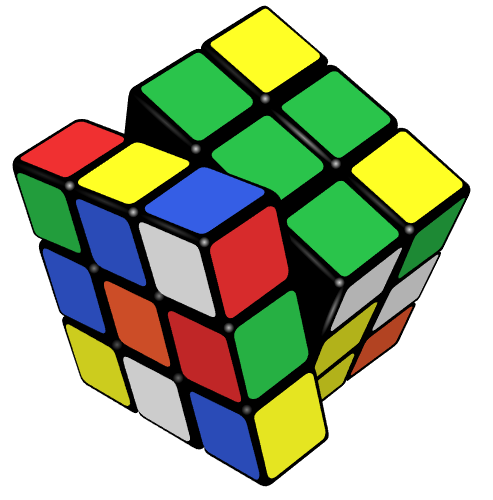
\includegraphics[width = 8cm]{weekly/week 14/despicable puzzle.png}
        \hspace{2em}
        \caption{Thanks to \href{https://commons.wikimedia.org/wiki/File:Rubik\%27s_cube.svg}{Wikipedia Commons!}}
        \label{fig:despicable}
    \end{figure}
    
    \begin{enumerate}
        \item How many possible configurations of the $3 \times 3$ Rubik's Cube are there?
        
        \item (\fullchili) In the context of a $3 \times 3$ cube, we say the puzzle is \textit{solved} if each face has $9$ tiles of the same color. Prove that if a corner has been twisted, the puzzle cannot be solved. Consider group theory.
        
        \item (\fullchili \hspace{1pt} $\times$ 2) Let the \textit{twisting number} of a Rubik's Cube be $C = 0$, where we add $1$ for each clockwise corner twist and subtract $1$ for each counterclockwise corner twist. Prove that if $C$ is odd, the puzzle cannot be solved.
    \end{enumerate}
    
\end{enumerate}

\newpage
\section{Geometry}
\begin{enumerate}[label=\textbf{G\arabic*}.]
    \item (\fullchili) \textbf{Dimension-travelling Circle} \newline
    Prove that the largest possible radius of a circle contained in an $n$-dimensional unit hypercube is
    \[ \frac{1}{2}\sqrt{\frac{n}{2}}. \]
    It may be helpful to consider the generalized parametric equation for a circle,
    \[ \overrightarrow{C} = \overrightarrow{a} + \overrightarrow{u}\cos t + \overrightarrow{v}\sin t, \]
    where $a, u, v$ are vectors satisfying $\lvert\lvert \overrightarrow{u} \rvert\rvert = \lvert\lvert \overrightarrow{v} \rvert\rvert$ and $u \cdot v = 0$ (both vectors are perpendicular).
\end{enumerate}

\newpage
\section{Number Theory}
\begin{enumerate}[label=\textbf{N\arabic*}.]
    \item \textbf{Recurring Divisibility} \newline
    Prove that the smallest integer greater than $(\sqrt{3} + 1)^{2n}$ is divisible by $2^{n+1}$ for all naturals $n$.
    
    \item \textbf{Collatz Conjecture Numero Duo (Aliquot Sequences)} \newline
    Let $s(n) = \sigma(n) - n$, where $\sigma(n)$ denotes the sum of the factors of $n$. Here, we have $3$ possible outcomes for what $s(n)$ could be.
    \[ \text{If } s(n) \begin{cases} < & n \text{ then $n$ is \textit{deficient}.} \\ = & n \text{ then $n$ is \textit{perfect}.} \\ > & n \text{ then $n$ is \textit{abundant}.} \end{cases} \]
    
    \begin{enumerate}
        \item If $n$ is a perfect number, we see that
        \[ s(n) = s(s(n)) = s(s(s(n))) = \dots. \]
        How many such $n$ can you find?
        
        \item (\halfchili) Suppose $a, b$ are relatively prime. Prove that $s(a)s(b) \leq s(ab)$.
        
        \item (\fullchili \hspace{1pt} $\times$ Open) Does there exist some $n$ such that the entire sequence below
        \[ s(n) < s(s(n)) < s(s(s(n))) < \dots \]
        is abundant?
    \end{enumerate}
    
\end{enumerate}

\end{document}
